% SQUARE \& CUBE ROOTS - WORKSHEET 0 (IN-CLASS INSTRUCTION)
\documentclass[12pt, letterpaper, fleqn]{article}

% ----------------------------------------------------------
% PACKAGES
% ----------------------------------------------------------
\usepackage{graphicx}
\usepackage{xcolor}
\usepackage[most]{tcolorbox}
\usepackage{amsmath, amssymb}
\usepackage{fancyhdr}
\usepackage[utf8]{inputenc}
\usepackage[T1]{fontenc}
\usepackage{enumitem}
\usepackage{geometry}
\usepackage{tikz}
\usepackage{needspace}
\usepackage{multicol}

\usetikzlibrary{arrows.meta, calc, positioning}

% ----------------------------------------------------------
% PAGE SETUP
% ----------------------------------------------------------
\usepackage{times}
\geometry{letterpaper, top=1.25in, bottom=1.25in, marginpar=0.5in}

% ----------------------------------------------------------
% HEADER / FOOTER
% ----------------------------------------------------------
\newcommand{\logowidth}{3cm}
\setlength{\headheight}{20pt}
\setlength{\footskip}{40pt}

\pagestyle{fancy}
\fancyhf{}
\fancyhead[C]{\small\bfseries Irrational Numbers \& Square/Cube Roots}
\fancyfoot[L]{\raisebox{2pt}{
\includegraphics[width=\logowidth]{../kss.png}}}
\fancyfoot[C]{\thepage}
\fancyfoot[R]{8.21.0}

\renewcommand{\footrulewidth}{0.2pt}

% ----------------------------------------------------------
% THEME COLOR
% ----------------------------------------------------------
\definecolor{customteal}{HTML}{2fbdb9}

% ----------------------------------------------------------
% HELPER MACROS
% ----------------------------------------------------------
\newcommand{\blank}{\underline{\hspace{2.2cm}}}
\newcommand{\blanklong}{\underline{\hspace{6.5cm}}}
\newcommand{\blankshorter}{\underline{\hspace{1.5cm}}}

% ----------------------------------------------------------
% DOCUMENT
% ----------------------------------------------------------
\begin{document}

\textbf{Name:} \underline{\hspace{5cm}}
\hfill
\textbf{Date:} \underline{\hspace{3cm}}\\

% ==========================================================
% SECTION 1: FOUNDATION
% ==========================================================
\begin{tcolorbox}[colback=customteal!20]
    \large\textcolor{black}{\textbf{Foundation: Roots and Irrational Numbers}}
\end{tcolorbox}

\vspace{3mm}

\noindent
Taking a root is the inverse operation of using an exponent.

\begin{itemize}
    \item \textbf{Square Roots ($\sqrt{x}$):} Asks "What number multiplied by \textit{itself} equals $x$?" For example, $\sqrt{25} = 5$ because $5^2 = 25$.
    \item \textbf{Cube Roots ($\sqrt[3]{x}$):} Asks "What number multiplied by itself \textit{three times} equals $x$?" For example, $\sqrt[3]{8} = 2$ because $2^3 = 8$.
    \item \textbf{Rational Numbers:} Can be written as a simple fraction (e.g., $1/2, 0.75, 4$). Perfect squares have rational roots (e.g., $\sqrt{9} = 3$).
    \item \textbf{Irrational Numbers:} Cannot be written as a simple fraction. The decimal goes on forever without repeating. If a number is NOT a perfect square, its square root is irrational (e.g., $\sqrt{10} \approx 3.16227...$). $\pi$ is also irrational!
\end{itemize}

\vspace{4mm}

% ==========================================================
% VISUAL REPRESENTATION
% ==========================================================
\begin{tcolorbox}[colback=white, colframe=black!25, boxrule=0.6pt, arc=4mm, left=6mm, right=6mm, top=5mm, bottom=5mm]

\textbf{Visual Representation: Geometry of Roots}

\medskip

\begin{center}
\begin{tikzpicture}[scale=0.8]

% Square
\draw[thick, fill=blue!10] (0,0) rectangle (2,2);
\node at (1,1) {Area = $9$};
\draw[<->] (0,-0.3) -- (2,-0.3) node[midway, below] {$x$};
\draw[<->] (-0.3,0) -- (-0.3,2) node[midway, left] {$x$};

\node[right] at (2.5, 1) {$x^2 = 9 \implies x = \sqrt{9} = 3$};

% Cube
\begin{scope}[shift={(8,0)}]
\draw[thick, fill=red!10] (0,0) rectangle (2,2);
\draw[thick, fill=red!10] (0,2) -- (0.8, 2.8) -- (2.8, 2.8) -- (2,2) -- cycle;
\draw[thick, fill=red!10] (2,0) -- (2.8, 0.8) -- (2.8, 2.8) -- (2,2) -- cycle;
\node at (1.4, 1.4) {Vol = $27$};

\node[below] at (1,0) {$s$};
\node[left] at (0,1) {$s$};
\node[above left] at (0.4, 2.4) {$s$};

\node[right] at (3.2, 1) {$s^3 = 27 \implies s = \sqrt[3]{27} = 3$};
\end{scope}

\end{tikzpicture}
\end{center}

\end{tcolorbox}

\vspace{4mm}

\newpage

% ==========================================================
% WORKED EXAMPLES
% ==========================================================
\begin{tcolorbox}[colback=customteal!20]
\large\textcolor{black}{\textbf{Estimating Irrational Roots}}
\end{tcolorbox}

\noindent
Since we can't write an exact fraction or terminating decimal for irrational numbers, we often have to \textbf{estimate} their value by placing them between two perfect squares on a number line.

\vspace{3mm}

\begin{tcolorbox}[colback=white, colframe=black!25, boxrule=0.6pt, arc=4mm, left=6mm, right=6mm, top=5mm, bottom=5mm]

\textbf{Worked Example 1: Estimating $\sqrt{40}$}

\medskip

\textbf{Problem:} Estimate the value of $\sqrt{40}$ to the nearest tenth.

\medskip

\textbf{Solution:}
\begin{itemize}
    \item \textbf{Step 1:} Find the perfect squares that $40$ is between. It's between $36$ and $49$.
    \item \textbf{Step 2:} Take the square roots. $\sqrt{36} = 6$ and $\sqrt{49} = 7$. So, $\sqrt{40}$ is between $6$ and $7$.
    \item \textbf{Step 3:} Look closer. $40$ is closer to $36$ than $49$ (it's 4 units away from 36, and 9 units away from 49). So the decimal will be less than $0.5$.
    \item \textbf{Step 4:} Estimate. Maybe $6.3$? Let's check $6.3^2 = 39.69$. Very close!
\end{itemize}

\end{tcolorbox}

\vspace{4mm}

% ==========================================================
% PRACTICE 1
% ==========================================================
\begin{tcolorbox}[colback=white!15, colframe=black, boxrule=1.5pt, arc=4mm, left=6mm, right=6mm, top=5mm, bottom=5mm]

\textbf{Guided Practice: Basic Operations}

\medskip

\noindent
\textbf{1.} Solve the equation: $x^2 = 64$.
\vspace{1.5cm}

\noindent
\textbf{2.} Solve the equation: $y^3 = -125$.
\vspace{1.5cm}

\noindent
\textbf{3.} Classify the following numbers as Rational or Irrational:
\begin{itemize}
    \item $\sqrt{100}$: \blankshorter
    \item $\sqrt{15}$: \blankshorter
    \item $\dfrac{2}{3}$: \blankshorter
\end{itemize}

\end{tcolorbox}

\newpage

% ==========================================================
% THINKING PROBLEM
% ==========================================================
\begin{tcolorbox}[colback=customteal!20]
\large\textcolor{black}{\textbf{Deeper Thinking: Number Line Placement}}
\end{tcolorbox}

\vspace{3mm}

\begin{tcolorbox}[colback=white!15, colframe=black, boxrule=1.5pt, arc=4mm, left=6mm, right=6mm, top=5mm, bottom=5mm]

\textbf{Deeper Thinking Problem 1: Ordering Real Numbers}

\medskip

\noindent
You are given the following set of numbers:
\[ \{ 3.5, \ \sqrt{10}, \ \pi, \ \sqrt{16}, \ \sqrt[3]{27} \} \]

\vspace{5mm}

\noindent
\textbf{a)} Convert or estimate the decimal value for each number. Show your approximations.

\vspace{4cm}

\noindent
\textbf{b)} Plot and label each number accurately on the number line below.

\vspace{1cm}

\begin{center}
\begin{tikzpicture}[x=2cm]
\draw[thick, <->] (2.5,0) -- (4.5,0);
\foreach \x in {3, 3.5, 4}
    \draw (\x,0.1) -- (\x,-0.1) node[below] {\x};
\end{tikzpicture}
\end{center}

\vspace{1cm}

\end{tcolorbox}

\end{document}
\end{document}
